\documentclass[stu,floatsintext]{apa7}
\usepackage[utf8]{inputenc}
\usepackage[american]{babel}
\usepackage{csquotes}
\usepackage{array}
\usepackage{tabularx}
\usepackage{pdflscape}
\usepackage[style=apa,sortcites=true,sorting=nyt,backend=biber]{biblatex}
\DeclareLanguageMapping{american}{american-apa}
\addbibresource{./Zotero.bib}
\linespread{1.0}

\title{Sample APA-Style Document Using the \textsf{apa7} Package}
\shorttitle{ }
\author{Jonas Colmsjö}
\affiliation{Gothenburg University, Department of Psychology}
\duedate{2021-XX-XX}
\course{PX1500 Bachelor Thesis, 15 credits, VT20YY}
\professor{Name of Professor}
\duedate{20YY-MM-DD}

\abstract{This demonstration paper uses the \textsf{apa7} \LaTeX\
  class to format the document in compliance with the 7th Edition of
  the American Psychological Assocation’s \textit{Publication Manual.}
  The references are managed using \textsf{biblatex}.}
\keywords{APA style, demonstration}
\authornote{The author can be reached at i@gizur.com}

\begin{document}
\maketitle

We begin with \textcite{thaler_nudge_2008}.  We can also cite this work in
parenthesis, like this: \parencite{thaler_nudge_2008}.
A three-author paper \parencite[e.g.,][]{anicich_hierarchical_2015} lists all
three authors for the first citation, then only the first author
on all subsequent citations \parencite{anicich_hierarchical_2015}.
Note the use of five heading levels throughout this demonstration
Method section.

\section{Method}
\subsection{Participants}
We had a lot of people in this study, see Figure \ref{fig:Figure1}.

\begin{figure}[h]
  \caption{ This is my figure caption.}
    \label{fig:Figure1}
  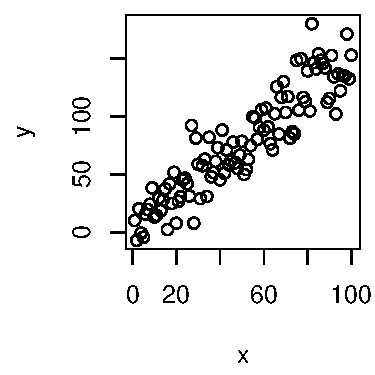
\includegraphics{./Figure1.pdf}
\end{figure}

\subsection{Materials}
Several materials were used for this project.  Some of them were
already created for prior research.

\subsubsection{Paper-and-Pencil Instrument}
We used an instrument that we found to be highly successful.

\paragraph{Reliability}
The reliability of this instrument is extraordinary.

\paragraph{Validity}
We now discuss the validity of our instrument.

\subparagraph{Face validity} The face validity is exceptionally
strong.  Everyone should be impressed.

\subparagraph{Construct validity} Also very strong.

\subsection{Design}
This section describes the study’s design.

\subsection{Procedure}
The procedure was fairly straightforward, yet required
attention to detail.

\section{Results}
Table \ref{tab:ComplexTable} contains some sample data.  Our
statistical prowess in analyzing these data is unmatched.

\begin{table}[htbp]
\vspace*{2em}
  \begin{threeparttable}
    \caption{A Complex Table}
    \label{tab:ComplexTable}
    \begin{tabular}{@{}lrrr@{}}           \toprule
      Distribution type  & \multicolumn{2}{l}{Percentage of} & Total number    \\
                         & \multicolumn{2}{l}{targets with}  & of trials per   \\
                         & \multicolumn{2}{l}{segment in}    & participant     \\ \cmidrule(r){2-3}
                                     &  Onset  &  Coda             &           \\ \midrule
      Categorical -- onset\tabfnm{a} &  100    &    0              & 196       \\
      Probabilistic                  &  80     &   20\tabfnm{*}    & 200       \\
      Categorical -- coda\tabfnm{b}  &  0      &  100\tabfnm{*}    & 196       \\ \midrule
    \end{tabular}
    \tablenote{All data are approximate.
      \tabfnt{a}Categorical may be onset.
      \tabfnt{b}Categorical may also be coda.
      \tabfnt{*}\textit{p} < .05.
      \tabfnt{**}\textit{p} < .01.}
  \end{threeparttable}
\end{table}

\section{Discussion}
This is a lengthy and erudite discussion.  It demonstrates amazing
skill in interpreting the results for the masses.

\printbibliography

\appendix

\section{Background scales}
\label{app:appendix_a}

The scales presented here were used to collect background information. The order
for the scales was randomized. The order the items within each scale was presented
was also randomized. An additional item was a attention check was added to the PFC-B questionnaire.
The SES questionnaire contained an additional attention check.

\subsection{PSA \parencite{grant_giving_2008,gneezy_paying_2012}} \label{app:psa}
Please indicate how much you agree or disagree with each of the following statements:
\begin{enumerate}
    \item I see myself as helpful.
    \item I see myself as selfish.
    \item I see myself as caring.
    \item I see myself as generous
    \item I regularly go out of my way to help others.
\end{enumerate}

\end{document}
